\documentclass[a4paper, 12pt]{article}

%%% SST LAB PROTOCOLL PREAMBLE
%%% 2019
%%%%%%%%%%%%%%%%%%%%%%%%%%%%%%%


%%% PACKAGES
%%%%%%%%%%%%%%%%%%%%%%%%%%%

\usepackage[ngerman]{babel}

\usepackage[utf8]{inputenc}
\usepackage{amsmath}
\usepackage{pgfplots}
\usepackage{tikz}
\usepackage[many]{tcolorbox}
\usepackage{graphicx}
\graphicspath{ {./graphics/} }
\usepackage{pdfpages}
\usepackage{dashrule}
\usepackage{float}
\usepackage{siunitx}
\usepackage{trfsigns}
\usepackage{booktabs}
\usepackage[european]{circuitikz}

%%% DOCUMENT GEOMETRY
%%%%%%%%%%%%%%%%%%%%%%%%%%%

\usepackage{geometry}
\geometry{
 a4paper,
 total={0.6180339887498948\paperwidth,0.6180339887498948\paperheight},
 top = 0.1458980337503154\paperheight,
 bottom = 0.1458980337503154\paperheight
 }
\setlength{\jot}{0.013155617496424828\paperheight}
\linespread{1.1458980337503154}

\setlength{\parskip}{0.013155617496424828\paperheight} % paragraph spacing


%%% COLORS
%%%%%%%%%%%%%%%%%%%%%%%%%%%

\definecolor{red1}{HTML}{f38181}
\definecolor{yellow1}{HTML}{fce38a}
\definecolor{green1}{HTML}{95e1d3}
\definecolor{blue1}{HTML}{66bfbf}
\definecolor{hsblue}{HTML}{00b1db}
\definecolor{hsgrey}{HTML}{afafaf}

%%% CONSTANTS
%%%%%%%%%%%%%%%%%%%%%%%%%%%
\newlength{\smallvert}
\setlength{\smallvert}{0.0131556\paperheight}


%%% COMMANDS
%%%%%%%%%%%%%%%%%%%%%%%%%%%

% differential d
\newcommand*\dif{\mathop{}\!\mathrm{d}}

% horizontal line
\newcommand{\holine}[1]{
  	\begin{center}
	  	\noindent{\color{hsgrey}\hdashrule[0ex]{#1}{1pt}{3mm}}\\%[0.0131556\paperheight]
  	\end{center}
}

% mini section
\newcommand{\minisec}[1]{ \noindent\underline{\textit {#1} } \\}

% quick function plot
\newcommand{\plotfun}[3]{
  \vspace{0.021286\paperheight}
  \begin{center}
    \begin{tikzpicture}
      \begin{axis}[
        axis x line=center,
        axis y line=center,
        ]
        \addplot[draw=red1][domain=#2:#3]{#1};
      \end{axis}
    \end{tikzpicture}
  \end{center}
}

% box for notes
\newcommand{\notebox}[1]{

\tcbset{colback=white,colframe=red1!100!black,title=Note!,width=0.618\paperwidth,arc=0pt}

 \begin{center}
  \begin{tcolorbox}[]
   #1 
  \end{tcolorbox}
 
 \end{center} 
 
}

% box for equation
\newcommand{\eqbox}[2]{
	
	\tcbset{colback=white,colframe=hsblue!100!black,title=,width=#2,arc=0pt}
	
	\begin{center}
		\begin{tcolorbox}[ams align*]
				#1
		\end{tcolorbox}
		
	\end{center} 
	
}

% END OF PREAMBLE

%%%%%%%%%%%%%%%%%%%%%%%%%%%%%%%%%%%%%

\begin{document}

%%%%%%%%%%%%%%%%%%%%%%%%%%%%%%%%%%%%%
  
\includepdf{./titlepage/titlepage.pdf}
  \clearpage
  \setcounter{page}{1}
%%%%%%%%%%%%%%%%%%%%%%%%%%%%%%%%%%%%%

\section{Vorbereitungsaufgaben}
%%%%%%%%%%%%%%%%%%%%%%%%
% 1.1

\subsection{}

Da ein periodisches Signal vorliegt, kann es mithilfe der
Fourierreihe
\[
x(t) = \frac{a_0}{2} + \sum_{n=1}^{\infty}{a_n \cdot \cos{(n \omega_0 t)} + b_n \cdot \sin{(n \omega_0 t)}} 
\]

in seine diskreten Frequenzanteile $a_n$ und $b_n$ bei $n \cdot \omega_0$ zerlegt werden.
\[
a_n = \frac{2}{T} \cdot \int_T{x(t) \cdot \cos{n \omega_0 t} \dif t}
\]
\[
b_n = \frac{2}{T} \cdot \int_T{x(t) \cdot \sin{n \omega_0 t} \dif t}
\]

\noindent Die Rechteckfolge ist eine gerade Funktion, $x(t)=x(-t)$, weshalb die Koeffizienten $b_n = 0$ sind.

\begin{gather*}
  a_n = \frac{2}{T} \cdot \int_{-T/2}^{T/2}{...} 
  = \frac{2}{T} \cdot \int_{-\tau/2}^{\tau/2}{U_0 \cdot \cos{n \omega_0 t}
    \dif t}\\
  = \frac{4}{T} \cdot U_0 \cdot \int_{0}^{\tau/2}{\cos{n \omega_0 t} \dif t}\\
  = \frac{4}{T} \cdot U_0 \cdot \frac{1}{n \omega_0} \cdot \sin{n \omega_0 \cdot \frac{\tau}{2}}\\
  \intertext{mit $\omega_0 = 2 \pi / T$}
  a_n = \frac{2 U_0}{n \pi} \cdot \sin{(n \pi \cdot \frac{\tau}{T})}\\
  \intertext{durch Erweiterung mit $\tau/T$ in die Form $\sin(x)/x = Si(x)$ }\\
\end{gather*}

\eqbox{a_n = 2 U_0 \cdot \frac{\tau}{T} \cdot Si(n \pi \cdot \frac{\tau}{T}) }{0.618\textwidth}

\begin{figure}[H]
	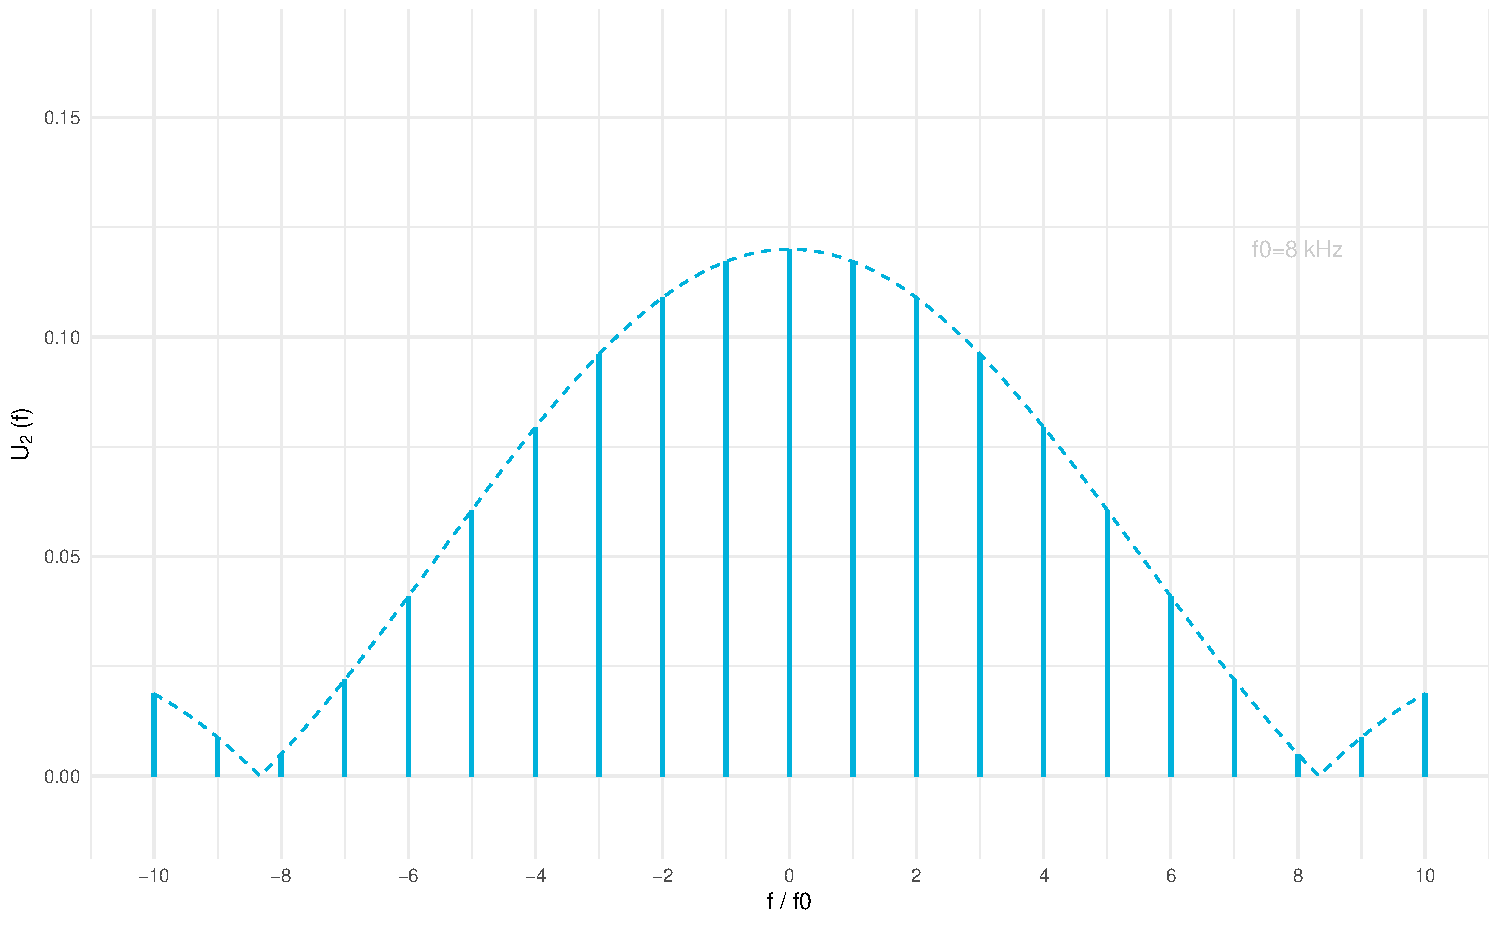
\includegraphics[width=\textwidth]{1_1/Si_8kHz}
  \caption{Teil des Spektrums der Rechteckimpulsfolge bei $T=1/8\,\si{\milli\second}$}
\end{figure}

\begin{figure}[H]
	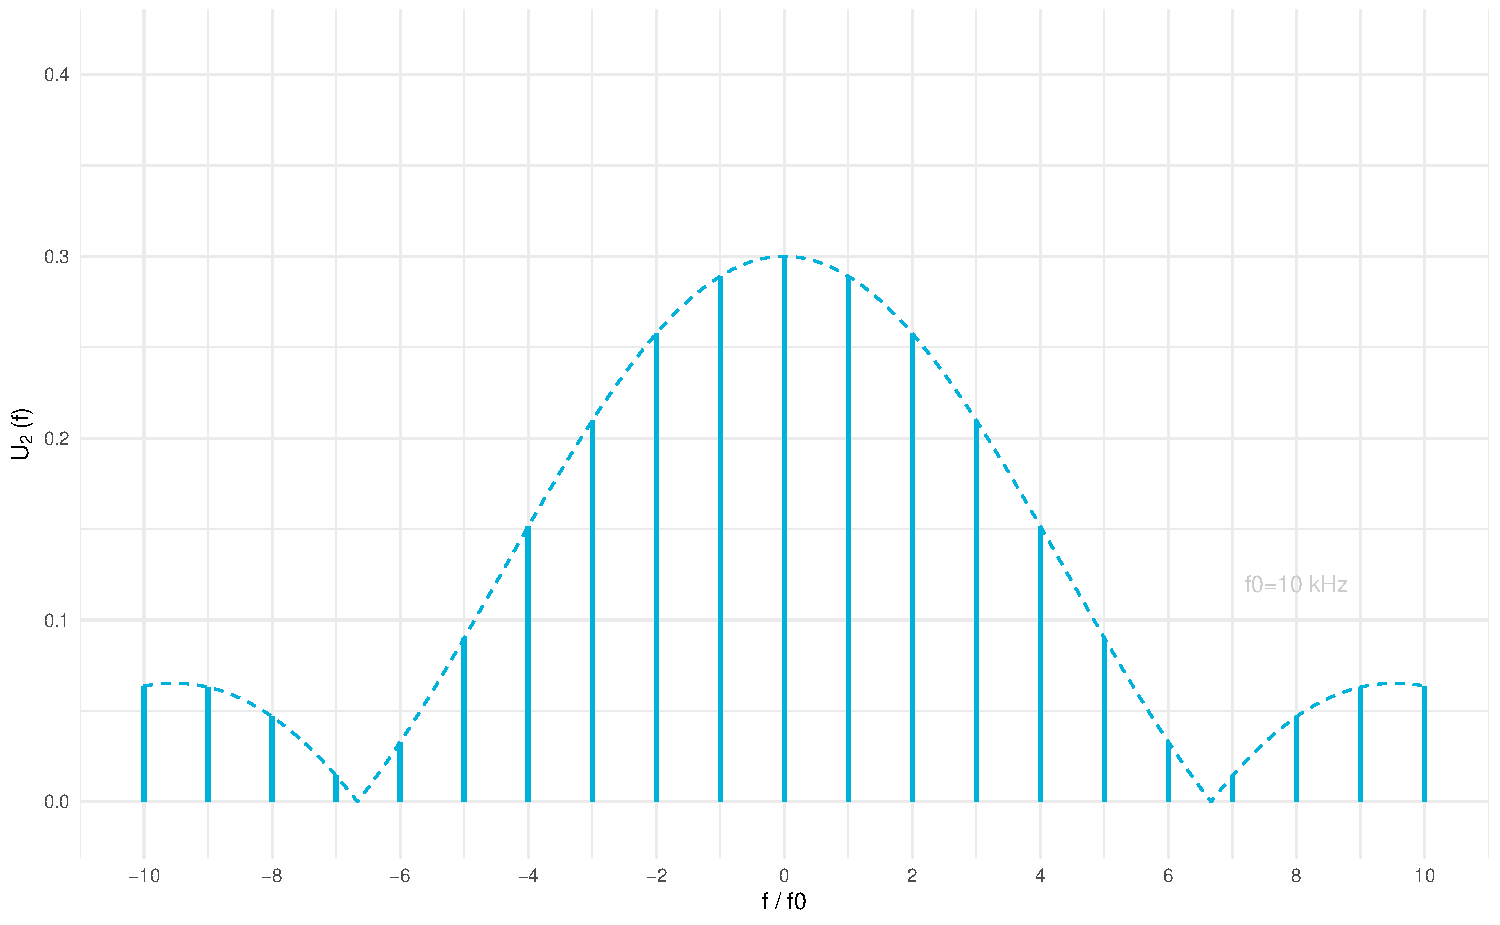
\includegraphics[width=\textwidth]{1_1/Si_10kHz}
  \caption{Teil des Spektrums der Rechteckimpulsfolge bei $T=1/10\,\si{\milli\second}$}
\end{figure}
%%%%%%%%%%%%%%%%%%%%%%%%
% 1.2

\subsection{}
Für die fehlerlose Signalabtastung muss die Abtastfrequenz $f_A$ mindestens
doppelt so groß sein wie die maximal im Signal auftretende Frequenz $f_{SMax}$ (Nyquist-Theorem).
\[
  f_A \geq 2\cdot f_{SMax}
\]

%%%%%%%%%%%%%%%%%%%%%%%%
% 1.3

\subsection{}

Die Multiplikation des Eingangssignals $u_1(t)$ mit dem Diracimpulskamm $u_0(t)$
führt auf eine Faltung im Zeitbereich.
\[
U_2(f) = U_1(f) * U_0(f)
\]
Die Fouriertransformation des Dirac-Kammes $U_0(f)$
führt ebenfalls auf einen mit der Abtastperiode gedämpften Dirac-Kamm
\[
  u_0(t) \,\, \laplace \,\, \frac{1}{T_a} \cdot \sum_{k=-\infty}^{\infty}{\delta{(f - k
      \cdot \frac{1}{T_a})}}
\]

Die Faltung einer Funktion $f(x)$ mit einem Diracimpuls $\delta(x)$ führt zur Verschiebung dieser
Funktion an die Stelle des Diracs $B$ und Wichtung der Funktion mit dem Faktor $a$
\begin{equation}
\label{eq:1}
  f(x) * a \cdot \delta(x - B) = a \cdot f(x - B)
\end{equation}

Da ein Diracimpulskamm lediglich eine Summe mehrerer Diracimpulse ist, kann man
die Linearität des Faltungsintegrals ausnutzen
\begin{gather*}
  U_2(f) = U_1(f) * U_0(f)\\
  = \int_{-\infty}^{\infty}{U_1(F) \cdot U_0(F - f) \dif F}\\  
  = \frac{1}{T_a} \cdot \int{U_1(F) \cdot \sum_{k=-\infty}^{\infty}{\delta((F-f) - k
      \cdot \frac{1}{T_a})} \dif F }\\
  = \frac{1}{T_a} \cdot \left( \cdots + \underbrace{
      \int{U_1(F) \cdot \delta{(F-f)}}
    }_{\textrm{Gl. } (1)}
    +
    \underbrace{
      \int{U_1(F) \cdot \delta{((F-f) - \frac{1}{T_a})}}
      }_{\textrm{Gl. } (1)}
      + \cdots \right)
\end{gather*}

Es ergibt sich also die Summe der Faltungen der Funktion $U_1(f)$ mit den einzelnen
Diracimpulsen des Kammes, also im Falle des Frequenzbereiches die periodische Verschiebung
des Spektrums $U_1(f)$ um die Werte $k \cdot 1/T_a$.




\begin{figure}[H]
	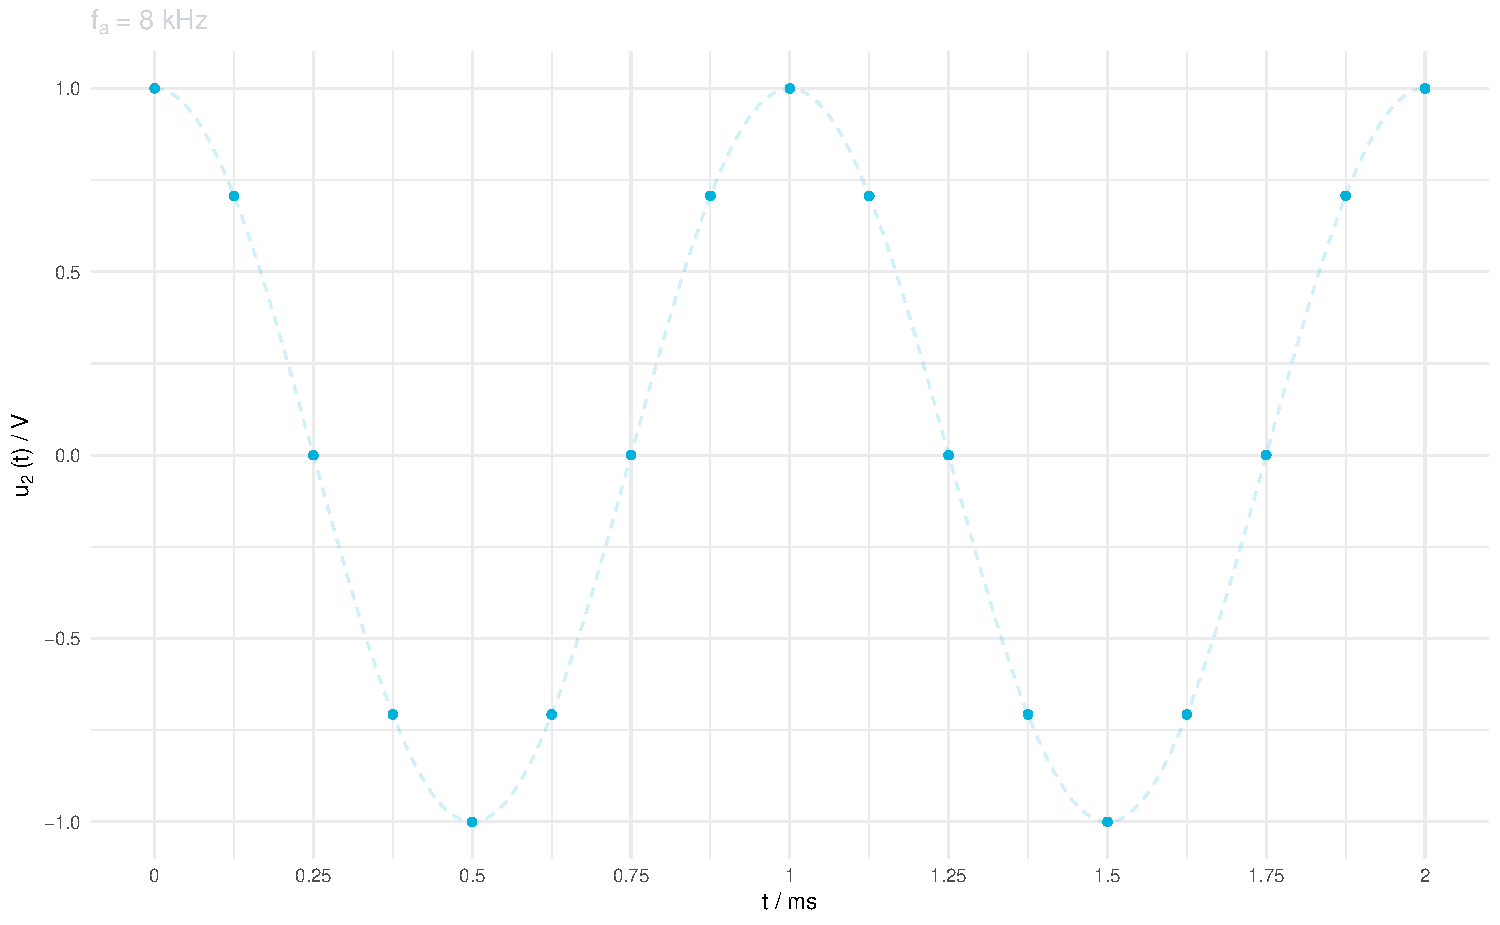
\includegraphics[width=\textwidth]{1_2/1_2_Abtast_8kHz_ZB}
  \caption{Zwei Perioden des Eingangssignals abgetastet mit $f_a=8\,\si{\kilo\hertz}$}
\end{figure}

\begin{figure}[H]
	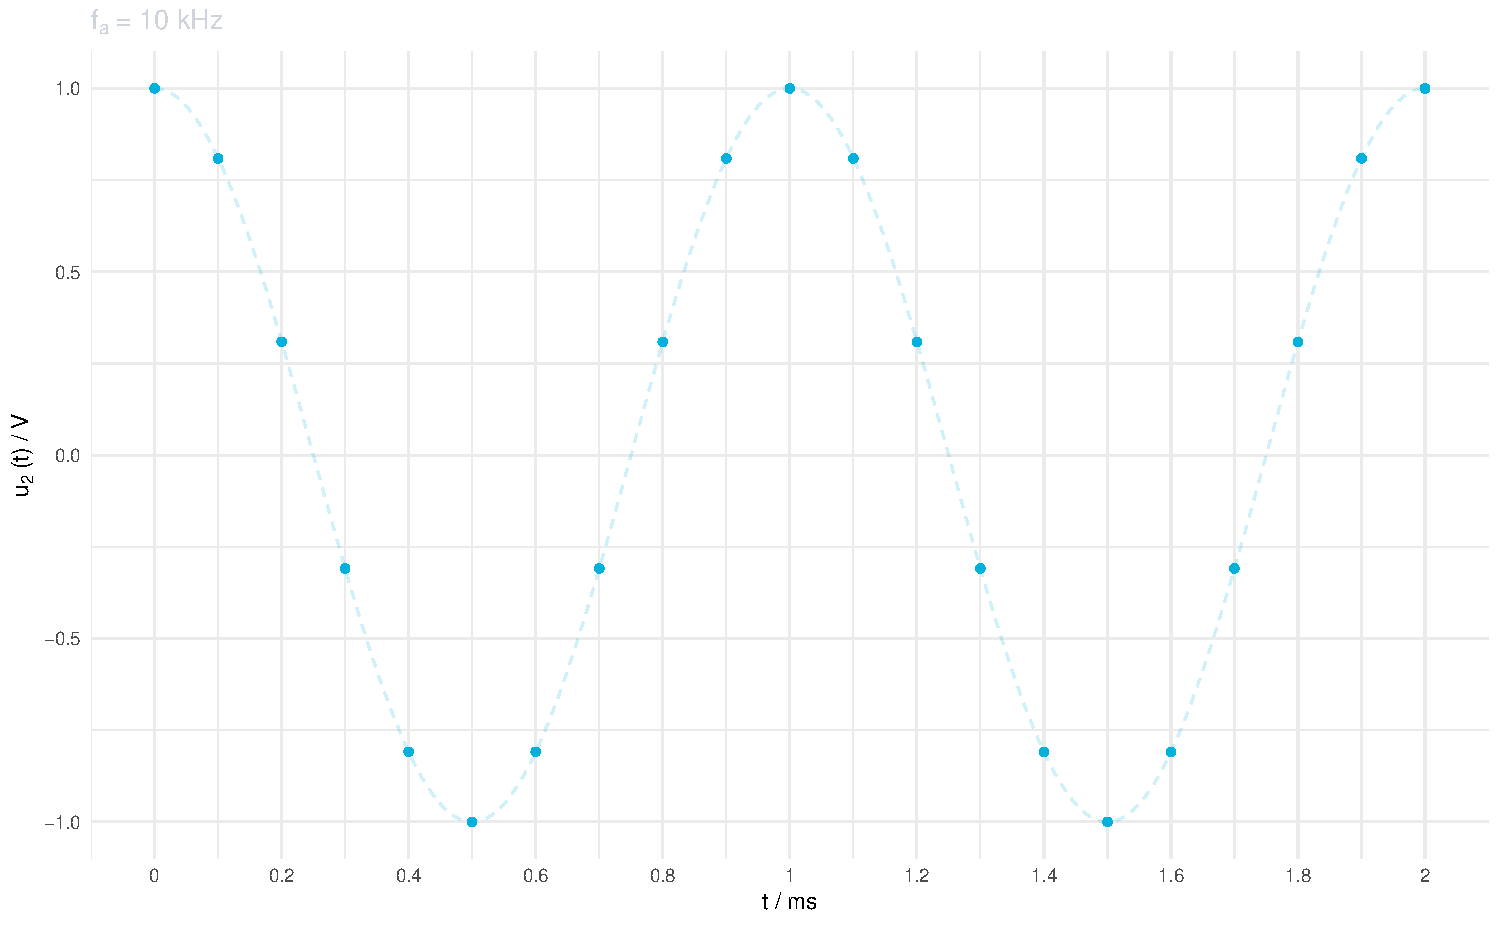
\includegraphics[width=\textwidth]{1_2/1_2_Abtast_10kHz_ZB}
  \caption{Zwei Perioden des Eingangssignals abgetastet mit $f_a=10\,\si{\kilo\hertz}$}
\end{figure}





\section{Versuchsaufgaben}


\end{document}
